\documentclass[titlepage]{jarticle}
%\usepackage{type1cm}
\usepackage{outline-ec}
\usepackage{amsmath,amssymb,verbatim,ascmac,multicol}
\usepackage{tabularx}
\usepackage{url}
\usepackage[hang,small,bf]{caption}
\usepackage[subrefformat=parens]{subcaption}

%\usepackage{multirow}
% dvioutで確認する場合は以下を有効にする
%\usepackage[dviout]{graphicx,color}
% pdf化する場合は以下を有効にする
\usepackage[dvipdfmx]{graphicx,color}

\captionsetup{compatibility=false}
\captionsetup[subfigure]{labelformat=simple}
\renewcommand{\thesubfigure}{(\alph{subfigure})}
%
% --------------------------------------------------------------------------
% 図表番号の後の:を削除
%
\makeatletter
\long\def\@makecaption#1#2{% #1=図表番号,#2=キャプション本文
  \sbox\@tempboxa{#1 \hskip0.5zw #2}% 図表番号とキャプションの間のスペース 0.5zw
  \ifdim \wd\@tempboxa >\hsize
    #1 #2\par
  \else
    \hb@xt@\hsize{\hfil\box\@tempboxa\hfil}
  \fi}
\makeatother

\氏名{本間 三暉}			%% 自分の氏名
\出席番号{35}					%% 出席番号
\研究室名{視覚情報処理研究室}			%% 研究室名
\指導教官{高橋 章}			%% 指導教員名

\発表番号{B\;--\;2}
\研究題目{単一視点による人物の全身運動の三次元計測について}

\アブストラクト{
a
}

\begin{document}
\maketitle

\section{研究背景・目的}
情報通信技術や処理速度の向上により機械学習を活用して効率化を図る動きが様々な分野で広がっている.
本研究室で行っている骨格推定の分野でも機械学習を活用し,%一台の入力装置や少ないセンサから
少ない情報から三次元の骨格推定を行えるオープンソースが増えている.



そこで本研究では一台の入力装置で三次元骨格推定を行う機械学習を活用した現行の方法を行う.
そして,動作の緩急やオクルージョンというカメラの手前にある物体に計測する箇所が隠れてしまい計測の信頼度が下がってしまう状態の有無について,それぞれの方法の精度を定量的に比較する.
\section{研究内容}
% \subsection{人の動作の計測方法}
%
人の動作の三次元計測を行うには,画像処理による方法やモーションセンサによる方法がある.%それぞれの方法について簡単にまとめたものを表\ref{3D_1}に示す.
% 画像処理による方法では画像から人の骨格を推定することで人の動作を解析できる.
画像処理による三次元骨格推定は撮影するカメラに,色情報を記録できる一般的なRGBカメラを用いて解析する方法(\ref{RGB_sec})と,
カメラと物体の距離を測ることができるRGBDカメラを用いて解析する方法(\ref{RGBD_sec})がある.

モーションセンサによる方法は,光学式や慣性式などがある.
光学式は体表面にマーカーを取り付けそのマーカーを複数台のカメラで取り込むことで骨格を推定する.
慣性式は加速度,角速度,方位を測定できるセンサを体表面の指定箇所に取り付けることで骨格を推定する.

市販の入力デバイスを使用し,PCで処理可能で専用の計測空間が不要な方法について性能を比較評価する.
% \begin{table}[t!]
%   \centering
%   \caption{動作を計測する方法の種類と特徴}
%   \begin{tabular}{l|ll|ll}
%     \hline
%                   & \multicolumn{2}{c|}{\small{カメラ}}       & \multicolumn{2}{c}{\small{モーションセンサ}}                                                     \\ \cline{2-5}
%                   & \multicolumn{1}{c|}{\small{RGB}}       & \small{RGBD}                         & \multicolumn{1}{c|}{\small{光学式}} & \small{慣性式}    \\ \hline
%     \small{センサ装着} & \multicolumn{1}{c|}{\small{不要}}        & \small{不要}                           & \multicolumn{1}{c|}{\small{必要}}  & \small{必要}     \\
%     \small{外から撮影} & \multicolumn{1}{c|}{\small{必要}}        & \small{必要}                           & \multicolumn{1}{c|}{\small{必要}}  & \small{不要}     \\
%     \small{必要台数}  & \multicolumn{1}{c|}{\small{1$\sim$数台}} & \small{1台}                           & \multicolumn{1}{c|}{\small{複数台}} & \small{0台}     \\ \hline
%     \small{計測方法}  & \multicolumn{1}{c|}{\small{MediaPipe}} & \small{Nuitrack}                     & \multicolumn{1}{c|}{\small{}}    & \small{mocopi} \\%%%これも怪しいけどね
%     \small{計測関節数} & \multicolumn{1}{c|}{\small{33個}}       & \small{19個}                          & \multicolumn{1}{c|}{\small{}}    & \small{27個}    \\
%     \hline
%   \end{tabular}
%   \label{3D_1}
% \end{table}
\begin{figure*}[t]
  \begin{tabular}{ccc}
    \begin{minipage}[]{0.3\hsize}
      \centering
      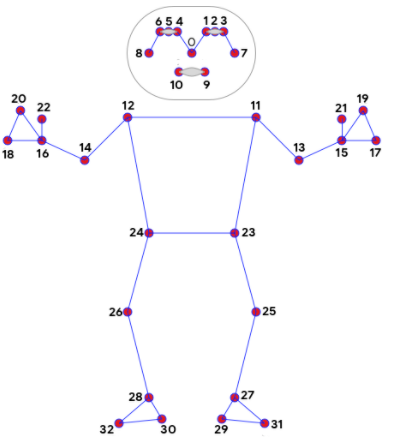
\includegraphics[height=45mm]{img/media.png}
      \subcaption{MediaPipe Poseで取得できる関節位置}
      \label{RGB} %%%後で変える
    \end{minipage}
    \hspace{0.03\columnwidth} % ここで隙間作成
    \begin{minipage}[]{0.3\hsize}
      \centering
      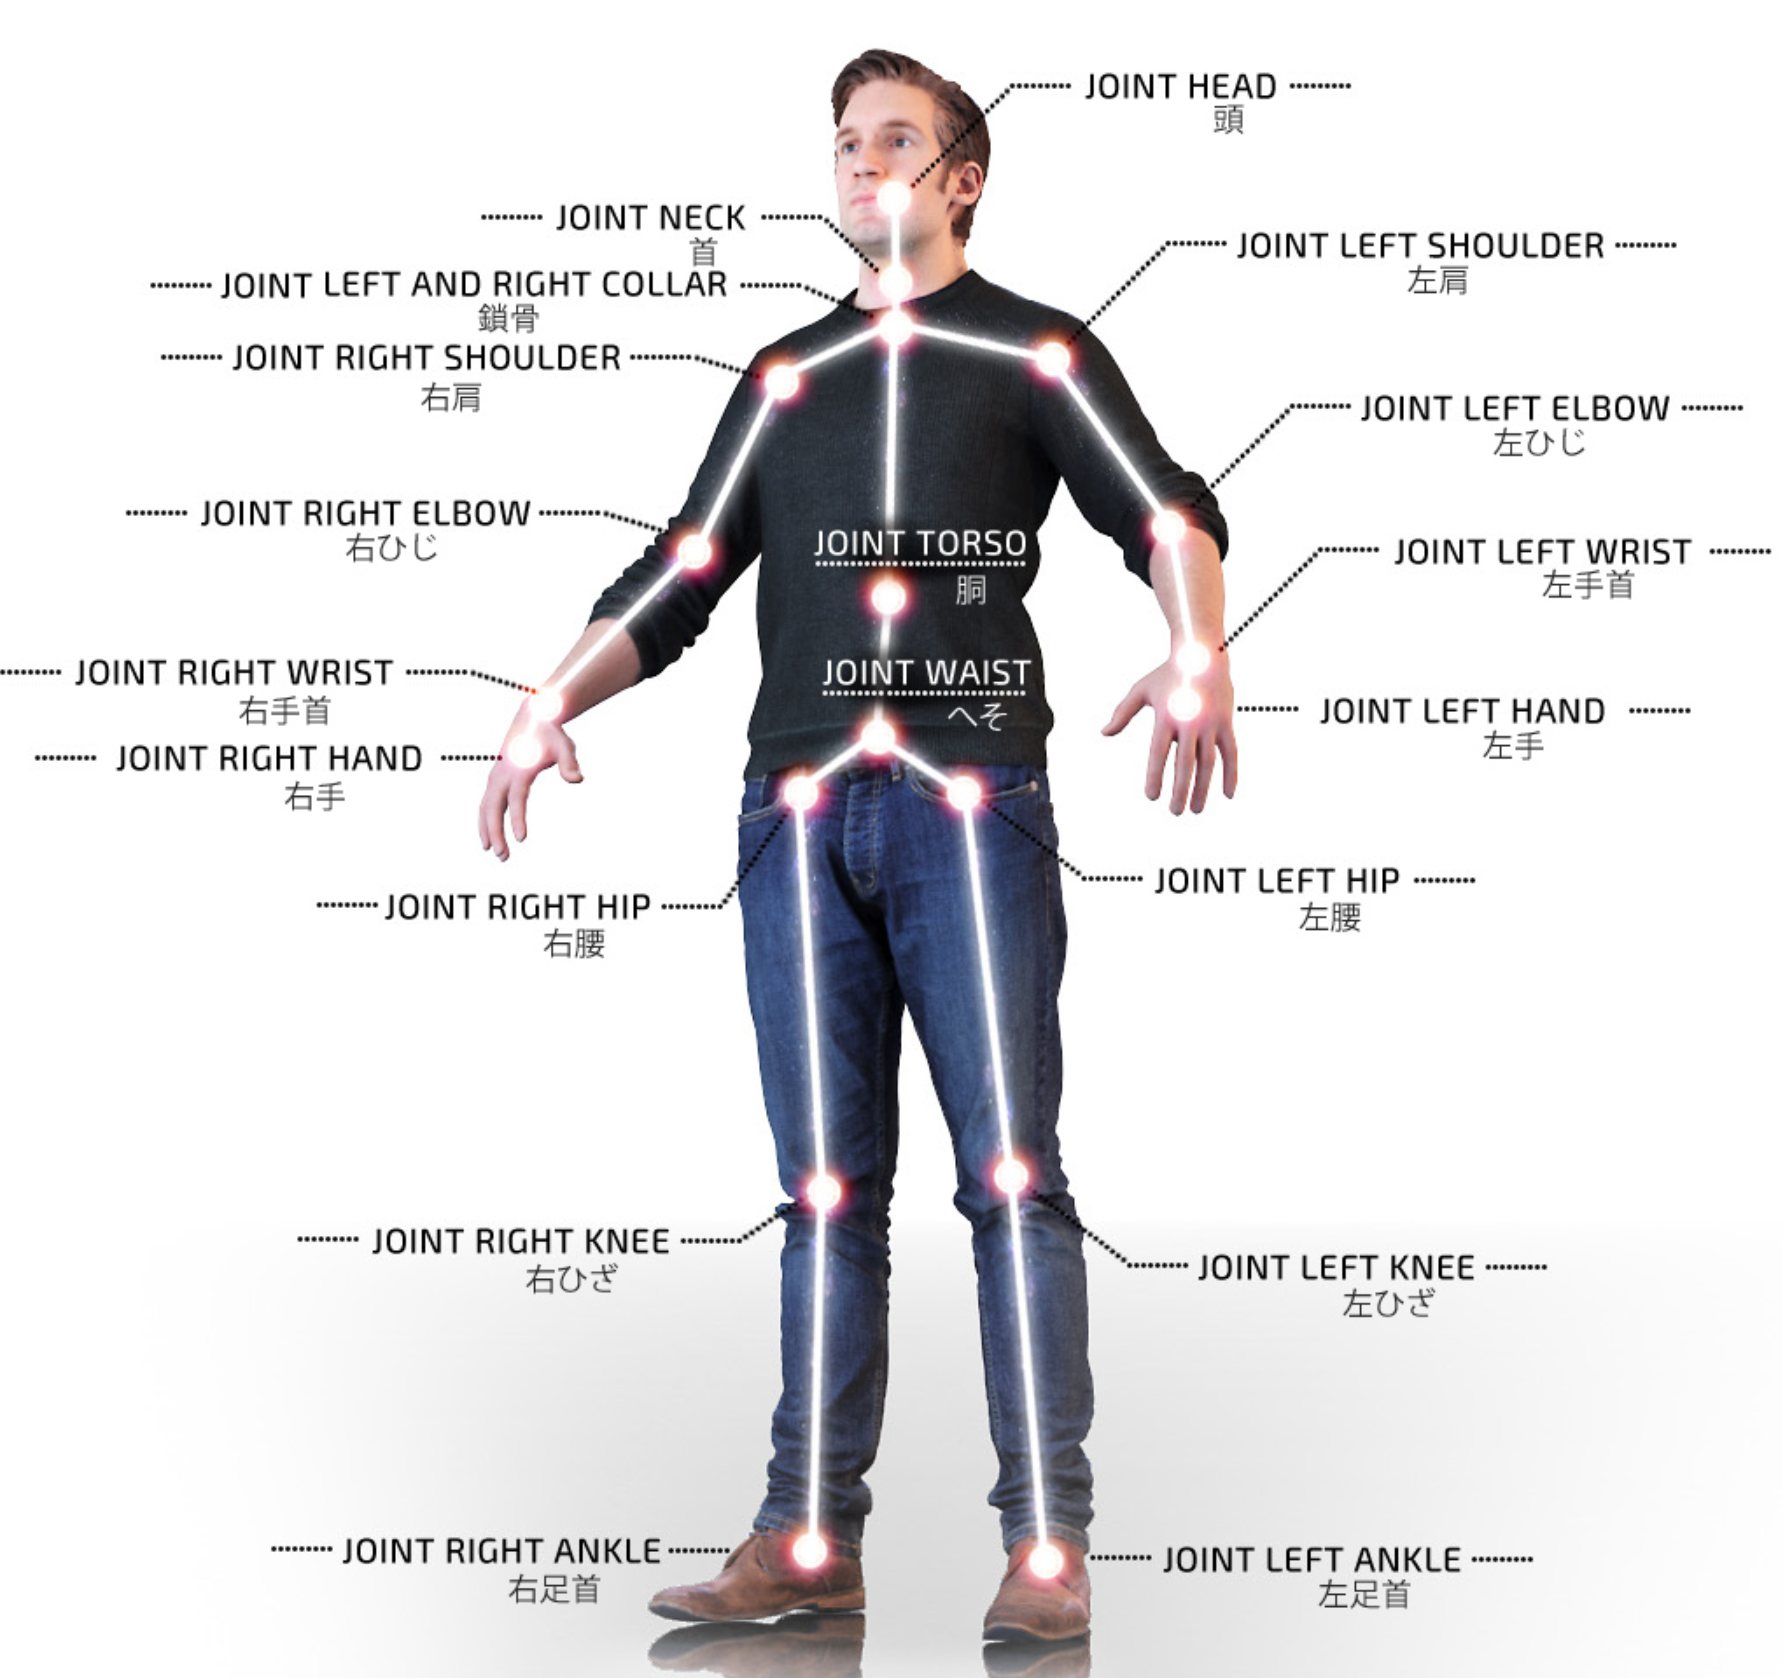
\includegraphics[height=45mm]{img/nuitrack.png}
      \subcaption{Nuitrackで取得できる関節位置}
      \label{RGBD} %%%後で変える
    \end{minipage}
    \hspace{0.03\columnwidth} % ここで隙間作成
    \begin{minipage}[]{0.3\hsize}
      \centering
      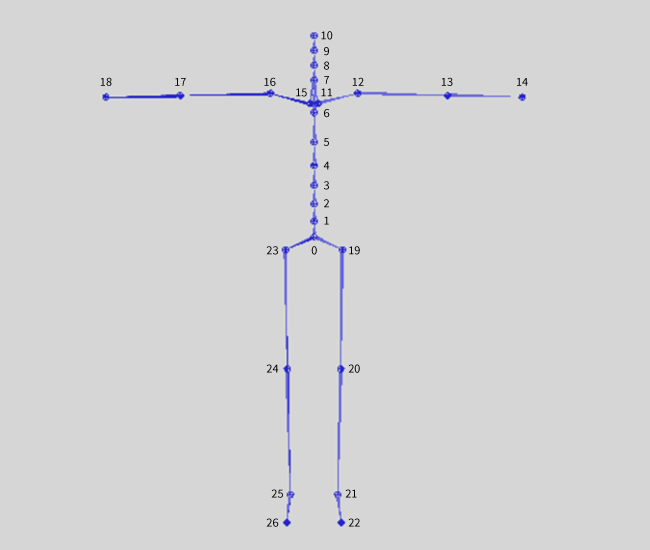
\includegraphics[height=45mm]{img/TechSpec_02.png}
      \subcaption{mocopiで取得できる関節位置}
      \label{mocopi} %%%後で変える
    \end{minipage}
  \end{tabular}
  \caption{取得できる骨格}
  \label{sokutei}
\end{figure*}
\subsection{RGBカメラ一台を用いた三次元骨格推定}\label{RGB_sec}
%
% 一台のRGBカメラで撮影した動画からMediaPipe Pose\cite{mediapipe}というライブラリを用いて処理することで骨格推定が行える.
%
% MediaPipeはGoogleが提供しているライブメディアやストリーミングメディア向けの機械学習ソリューションである.
% 顔認識や物体検出などが行えるライブラリがあり,計算コストが低くスマートフォンや組み込みPCなど資源の限られたハードウェアでも使用できる.
% また,その中でもMediaPipe Poseは動画から人間の姿勢を推論するライブラリで,
% 動画から図\ref{RGB}に示す全身の33個の関節の三次元位置または上半身の25個の関節の三次元位置を予測できる.
画像入力機器としてRGBDカメラであるRealSense D415を使用し,カラー画像を入力として図\ref{RGB}に示す33個の関節が取得できる,Googleが提供するオープンソースの機械学習ライブラリMediaPipe Poseで三次元計測を行う.
\subsection{RGBDカメラで行う三次元骨格推定}\label{RGBD_sec}
% kinectSDK\cite{kinectSDK}のようなデバイス専用のソフトウェアや,Nuitrack\cite{nuitrack}などのオープンソースを開発ライブラリに用いて処理することによってアプリケーションを作成できる.
% RGBDカメラを用いて骨格推定をする際に一般的という理由からNuitrackを使用する.
% Nuitrackは3DiVi Incが開発した三次元トラッキングミドルウェアで,RealSense D400シリーズやOrbbec Astraシリーズ等のRGBDカメラで骨格推定が可能であり,
% 図\ref{RGBD}に示す全身の19個の関節部分のトラッキングが可能である.
%
画像入力機器としてRGBDカメラであるRealSense D415を使用し,カラー画像と深度情報を入力として図\ref{RGBD}に示す19個の関節が取得できる,3DiVi Incが提供するNuitrackで三次元計測を行う.
\subsection{慣性式モーションキャプチャの三次元骨格推定}
% 画像処理による方法の精度を比較する際,画像処理とは独立した方法取得した骨格を基準としないと特定の方法に有利な結果が出てしまう可能性がある.
% そのため,画像処理とは独立した方法としてモーションキャプチャデバイスmocopiを用いて計測する.
%
% mocopiとは,市販のモーションキャプチャデバイスで両手,両足,頭,腰の計6か所に小型センサを装着してリアルタイムに三次元計測を行うことができる.
% 6つの小型センサで測定しているため肘や膝などの関節部の屈曲を正確に表現することはできないが,mocopiのセンサはそれぞれ3つの自由度を持つ加速度センサと角度センサで測定しており,
% 機械学習を用いることで,\ref{mocopi}に示すような肘や膝などの関節部を含めた全身の27個の関節位置を推定している.
慣性式のモーションキャプチャとしてそれぞれ3つの自由度を持つ加速度センサと角度センサを持つ小型センサ6つを両手,両足,頭,腰につけて,図\ref{mocopi}に示す27個の関節が取得できるmocopiを用いて三次元計測を行う.
\subsection{キャリブレーション}
計測方法により,座標系やスケールに違いが出たり,時間遅れが発生するため同期が必要である
そのため,座標系やスケール,処理により発生した時間遅れを統一するためのキャリブレーションを行う必要がある.

キャリブレーションの方法として計測前に2つの動作を行う.
1つ目が両腕を水平に広げるポーズである.このポーズをしたときの両手首の距離を元にスケールを合わせる.
また,へその位置を原点として,頭に向かう方向をz軸,右手から左手に向かう方向をx軸,これらの軸と直交する方向をy軸として座標系を定める.

2つ目が両手を胸の前であわせるポーズである.このポーズをしたときは両手首が最接近しているので,このタイミングを基準としてフレームのズレを合わせる.
\section{研究結果}
\subsection{実験方法}
RGB,RGBDの情報を撮るカメラにはIntel RealSense Depth Camera D415を使用し,慣性式のモーションキャプチャにはmocopiを使用した.
カメラの解像度は640$\times$360px,フレームレートは60fpsである.
実験には明るい室内で撮影した動画を使用した.

% 全身運動をしている人物一人に対して計測を行い,mocopiのセンサの位置に当たる両手,両足,頭,腰の計6ヶ所に関して,画像処理を用いた三次元骨格推定で得られた座標との誤差を比較することで精度を評価する.
全身運動をしている人物一人に対して計測を行い,体の部位の恒常性について比較する.
\subsection{解析結果}



\section{まとめ}
RGBDによる方法では現在問題の修正中である.
\begin{thebibliography}{99}
  \small{
    \bibitem{mediapipe}{
      Google,``mediapipe'',\\
      \url{https://developers.google.com/mediapipe}
    }




  }
\end{thebibliography}
\rightline{URLは2023年10月4日にアクセス}
\end{document}